\rhead{Dijagram prelaza stanja za objave}
\section{Dijagram prelaza stanja za objave}
\par Svaka objava može da se nalazi u 6 različitih stanja: \textit{kreirana}, \textit{odbijena},
\textit{prihvaćena}, \textit{sakrivena}, \textit{udomljen} i \textit{privremen smeštaj}. 
Stanja \textit{prihvaćena}, \textit{udomljena} i \textit{privremen smešta} su vidljivi za sve korisnike,
dok \textit{volonter} može da vidi objave u stanju \textit{kreirana}, \textit{sakrivena}.
\par U nastavku je navedeno na koji način objava dolazi do određenog stanja, kao i dijagram prelaza stanja [Slika \ref{fig:state}].
\begin{figure}[h]
    \centering
    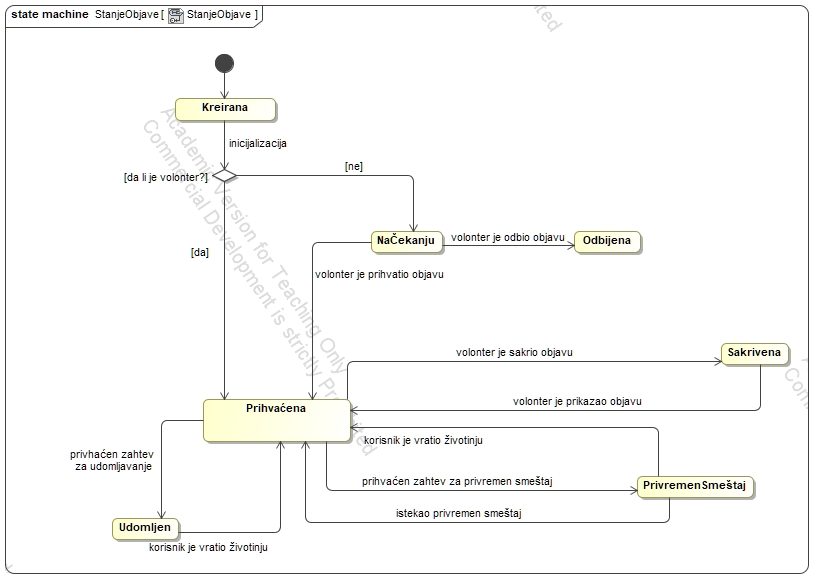
\includegraphics[width=\textwidth]{img/state.jpg}
    \caption{Dijagram prelaza stanja za objave}
    \label{fig:state}
\end{figure}
\begin{enumerate}
    \item \textbf{Kreirana}: početno stanje ako je objava kreirana od strane \textit{člana}.
    \item \textbf{Odbijena}: \textit{volonter} odbio objavu kreiranu od strane člana
    \item \textbf{Prihvaćena}: 
        početno stanje ako je objava kreirana od strane \textit{volontera}; 
        \textit{volonter} je prihvatio objavu kreiranu od strane člana;
        član koji je udomio životinju ili joj pružio privremen smeštaj odlučio da je vrati;
        privremen smeštaj je istekao;
        \textit{volonter} je otrio prethodno sakrivenu objavu
    \item \textbf{Sakrivena}: \textit{volonter} sakriva objavu
    \item \textbf{Udomljen}: prihvaćen je zahtev za udomljavanje
    \item \textbf{Privremen smeštaj}: prihvaćen je zahtev za privremen smeštaj
\end{enumerate}
\par Dijagram prelaza stanja sa slike \ref{fig:state} se može prevesti u klasni dijagram koji se nalazi
na slici \ref{fig:state-class}
\begin{sidewaysfigure}
    \centering
    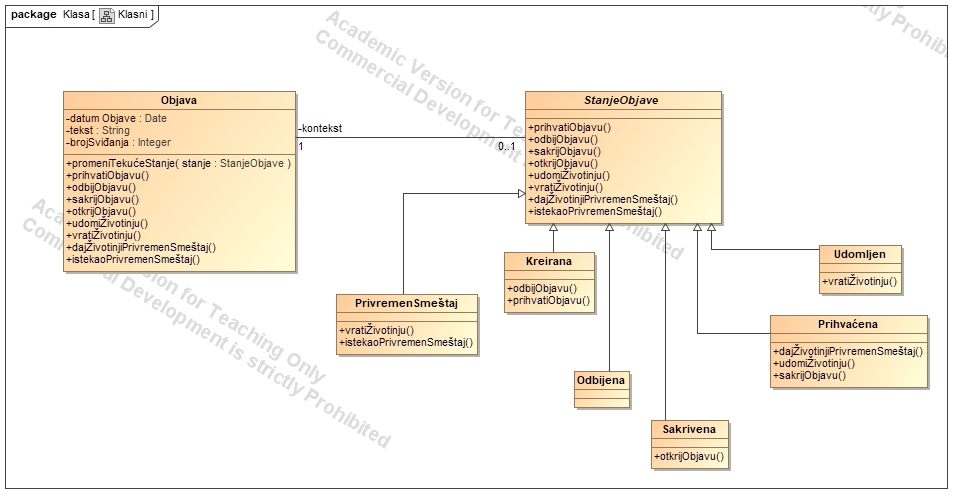
\includegraphics[height=0.5\textwidth, width=\textwidth]{img/state-class.jpg}
    \caption{Preveden dijagram prelaza stanja}
    \label{fig:state-class}
\end{sidewaysfigure}
